\documentclass{report}
\author{Alasdair Macindoe}
\date{}
\title{Work Package 5.2: A Report}
\usepackage{hyperref}
\usepackage{listings}
\usepackage{pgfplots}
\lstset{
  numbers = left,
  tabsize = 1,
  stepnumber = 1,
  breaklines=true,
}

\begin{document}
\maketitle

\section*{Acknowledgements}
We acknowledge financial support from the \href{http://opendreamkit.org/}{OpenDreamKit} \href{https://ec.europa.eu/programmes/horizon2020/}{Horizon 2020}
\href{https://ec.europa.eu/programmes/horizon2020/en/h2020-section/european-research-infrastructures-including-e-infrastructures}{European Research Infrastructures}
project (\href{http://cordis.europa.eu/project/rcn/198334_en.html}{\#676541}).
Further we would like to thank \href{https://www.cs.st-andrews.ac.uk/directory/person?id=mp397}{Dr Markus Pfeiffer} for his supervision and all his help
that was invaluable for this project.

\section*{Introduction}
Whilst enumerating finite semigroups is computationally expensive there are algorithms that can run - in a practical sense - faster than naively enumerating
the semigroup. One example of this algorithm was published in 1997 by Froidure and Pin\cite{fpin} (which will hereby be called the Froidure-Pin algorithm).
Unfortunately this algorithm does not run concurrently which is a problem for modern computational problems; thus this lead to another version of Froidure-Pin to be
published\cite{cfp} (which we will henceforth call the concurrent Froidure-Pin) which can run concurrently and for which a C++ implementation exists\cite{cfpcpp}.
\newline
\newline
\subsection*{Aim}
The aim of this project was to re-implement the concurrent Froidure-Pin algorithm in HPC-GAP\cite{GAP4} and analyse its scalability.
The full repository for this project can be found on Github\cite{project}. This code was then shared to the general public under
the GNY GPL v3 license.

\section*{Structure}
All the code can be located on Github\cite{project}. The following may be of interest:
\newline
\begin{description}
\item \texttt{README.md}: Installation and testing instructions
\item \texttt{versions.md}: Explanation of implementation details
\item \texttt{runtimes.md}: Raw data from experiments
\item \texttt{data.md}: Explanation of different semigroups for testing
\item \texttt{experiment.g}: File to run experiments
\item \texttt{gap/}: Various implementations
\item \texttt{tst/}: The test file
\end{description}

\section*{Failed Attempts and Approach}
This was a very challenging project, and there are many attempts before we arrived at \texttt{Version 2.1} which were failures.
The first attempt was creating in GAP the simplistic \texttt{naiveenumeration} variation, then from there work on implementing the
Froidure-Pin algorithm itself.
\newline
The real difficulty began with the concurrent Froidure-Pin algorthim which was written in some very dense mathematical notation.
We have an attempt \texttt{concurrentfp} where we completely misunderstood the algorithm, we have \texttt{Version 1.x} which whilst
do perform the job correctly and not truly concurrent at every stage and require locking.
The insights gained from these failures did allow us to produce \texttt{Version 2.1} which we are incredibly happy with.
\newline
Overall we feel like this approach was the most beneficial. Not only did it require learning about semigroups and GAP, but it allowed us
to start from the beginning and develop our way through the approaches done throughout the years and improve and learn ourselves from our failures.

\section*{Implementation}
\texttt{Version 2.1} is an exact implementation of the version given in the paper. Since the paper does not dictate what data structures should be used
the full implementation details can be found in \texttt{versions.md}. This gives very detailed overview of the algorithm and why it can run locklessly,
as well as the reasons for the specific data structures.

\section*{Analysis}
Please refer to \texttt{runtimes.md} for the raw data, only summaries are provided below.
\newline
All experiments are on implementation \texttt{Version 2.x}.

\subsection*{Experiment 1}
The aim of this experiment was to see the effect of increasing the number of core available without increasing the number of fragments.
\newline
We believe this was worth investigating because HPC-GAP's Task implementation is not guaranteed 1 to 1 with processes.
\newline
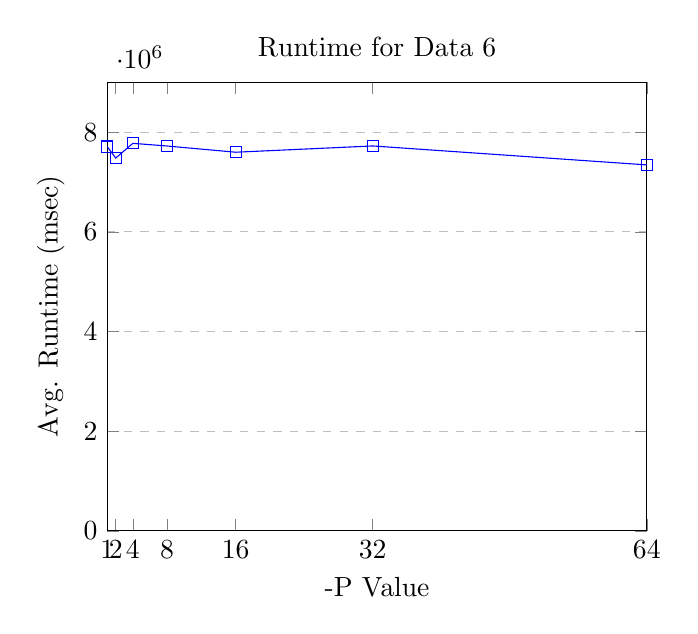
\begin{tikzpicture}
\begin{axis}[
    title={Runtime for Data 6},
    xlabel={-P Value},
    ylabel={Avg. Runtime (msec)},
    xmin=1, xmax=64,
    ymin=0, ymax=9000000,
    xtick={1, 2, 4, 8, 16, 32, 64},
    ymajorgrids=true,
    grid style=dashed,
]
 
\addplot[
    color=blue,
    mark=square,
    ]
    coordinates {
    (1, 7713242)(2, 7483817)(4, 7778529)(8, 7724759)(16, 7600084)(32, 7725967)(64, 7345427)
    };
 
\end{axis}
\end{tikzpicture}

From this we can see that there is no effect on the runtime when we just vary the number of core available without changing the number of fragments.

\subsection*{Experiment 2}
The aim of this experiment was to instead see how the number of fragments effects the runtime. We keep P = 32 for all attempts.
\newline
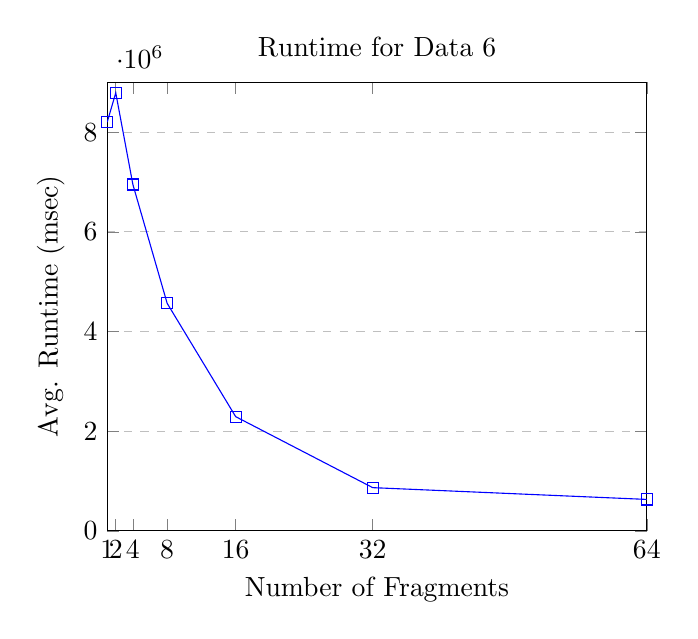
\begin{tikzpicture}
\begin{axis}[
    title={Runtime for Data 6},
    xlabel={Number of Fragments},
    ylabel={Avg. Runtime (msec)},
    xmin=1, xmax=64,
    ymin=0, ymax=9000000,
    xtick={1, 2, 4, 8, 16, 32, 64},
    ymajorgrids=true,
    grid style=dashed,
]
 
\addplot[
    color=blue,
    mark=square,
    ]
    coordinates {
    (1, 8202761)(2, 8792324)(4, 6952345)(8, 4567620)(16, 2291670)(32, 866321)(64, 629930)
    };
 
\end{axis}
\end{tikzpicture}
This very clearly has an impact even beyond the number of cores available. 

\begin{table}
\begin{tabular}{cc}
\multicolumn{1}{l}{\textbf{Cores}} & \multicolumn{1}{l}{\textbf{Speed up Percentage}} \\
1                                  & -                                                \\
2                                  & 107                                              \\
4                                  & 21                                               \\
8                                  & 35                                               \\
16                                 & 50                                               \\
32                                 & 63                                               \\
64                                 & 28                                              
\end{tabular}
\end{table}

This clearly shows that the rate of decrease in time becomes faster as we approach the number of cores and fragments being equal, it further shows that this rate decreases once we exceed that. Further experimentation may show that this trend reverses as we dramatically exceed our -P value. 
\newline
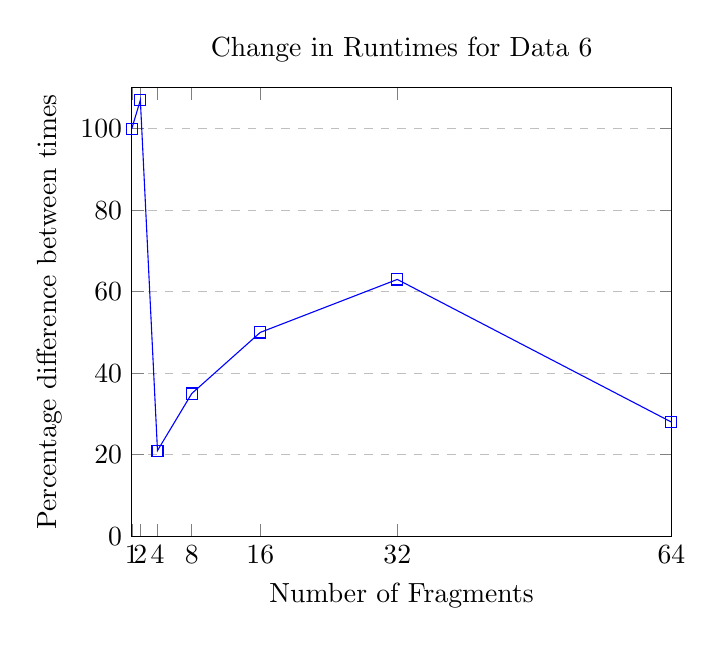
\begin{tikzpicture}
\begin{axis}[
    title={Change in Runtimes for Data 6},
    xlabel={Number of Fragments},
    ylabel={Percentage difference between times},
    xmin=1, xmax=64,
    ymin=0, ymax=110,
    xtick={1, 2, 4, 8, 16, 32, 64},
    ymajorgrids=true,
    grid style=dashed,
]
 
\addplot[
    color=blue,
    mark=square,
    ]
    coordinates {
    (1, 100)(2, 107)(4, 21)(8, 35)(16, 50)(32, 63)(64, 28)
    };
 
\end{axis}
\end{tikzpicture}
\section*{Contributions to HPC-GAP}
A bug in HPC-GAP was discovered which would cause a segmentation fault when an empty list was attempted to be migrated between tasks.
This was fixed by Dr Markus Pfeiffer\cite{hpcsol}.

\section*{Future Work}
We have identified some potential future works that could be done:

\begin{enumerate}
\item Fix any outstanding bugs and perform more significant testing
\item Covert data structures across to the HPC-GAP's datastructures package\cite{ds}
\item Investigate performance increases by using HPC-GAP's threads and processes API
\item Investigate performance increases in HPC-GAP's tasks system
\end{enumerate}

\section*{Conclusion}
In sum we have successfully implemented the concurrent Froidure-Pin algorithm several times in HPC-GAP and compared their scalability.
Additionally we have identified bugs that exist within HPC-GAP and identified future work that could be conducted in this area.
\newline
We further believe that the skills honed here will allow us to make stronger Computer Scientists and software engineers.
\newline
The experimentation clearly shows that the algorithm's runtime scales reasonably well with large number of cores with the most dramatic speed ups occurring as we near the number of available cores. 


\bibliographystyle{plain}
\bibliography{citations}
\end{document}
